\patternOne

\subsection*{Context}

Visually appealing course materials are a goal for many educators and are appreciated by students. 

Graphically designed course materials are appealing for sighted people. Graphics support the content to be taught. 

\ac{wysiwyg} tools such as Word or PowerPoint make it very easy to place graphics almost anywhere. 

\subsection*{Problem}

\begin{itshape}

Graphics are usually not accessible for the visually impaired. 
Text within graphics cannot be extracted by assistive tools.

\end{itshape}
    
    



\subsection*{Solution}

\begin{sol}
Extract the core content of teaching materials and represent it in a multi-directionally transformable format.
\end{sol}


First, eliminate all purely decorative graphics.
Analyze whether and what information is conveyed by typographic layout. 
Identify the graphics that carry the content to be taught.


This paper distinguishes between diagrams and graphics. 
In case of diagrams that adhere to a formal specification, such specifications typically define formats for textual representation. These structured formats enable systematic interpretation, transformation, and accessibility enhancement through computational means. 
Pattern \patternTwoInline presents solutions to gain accessibility for this type of diagrams. 

By contrast, graphics such as photographs, freehand drawings, and various other illustrative visualizations do not follow a formal specification. As a result, there is no underlying metamodel that can be leveraged to interpret or describe their content programmatically.
To make such unstructured graphics accessible—particularly for \ac{bvi} students haptic solutions are a promising approach. Tactile representations provide a means of conveying the structural and spatial properties of these graphics in a non-visual form, as introduced in pattern \patternThreeInline. 
 
Use simple, plain-text formats with minimal formatting whenever possible.
Plain text is easy to process with screen readers, Braille displays, and text-to-speech tools, making it more accessible for \ac{bvi} students. Markdown is a particularly suitable format. It offers basic yet effective formatting options and can be easily converted into various output formats such as HTML or PDF. However, purely textual materials may not be engaging for sighted students. They are accustomed to visually rich course materials, such as textbooks, handouts, and slide decks that follow well-designed layouts.
To address this, rendering tools can be used to convert the core content into visually appealing formats. By generating PDFs or web-based HTML documents, course materials can be presented in a way that meets the expectations of sighted learners—without compromising accessibility.

\subsection*{Examples}
 
Fig.~\ref{fig:questionmark} shows an example of a graphic that is used only for decoration. Such graphics do not carry any content. If they are to be used for visual reasons, the graphic should be labeled as purely decorative in the text-only version of the course materials.

\begin{figure}
    \centering
    \fbox{\includegraphics[page=3, width=0.12\linewidth]{img/out.pdf}}
    \caption{Solely decorative image}
    \label{fig:questionmark}
\end{figure}



Fig.~\ref{fig:freehand} shows an example where two small pictures are freely positioned on a slide. They illustrate the explanatory text left of them. However, they contribute to the content. Arrows point to the words "Dog" and "Human". The arrows shall visualize the  relationships "generalization" and "specialization" between classes in object-oriented programming. 

\begin{figure}[ht!]
    \centering
    \fbox{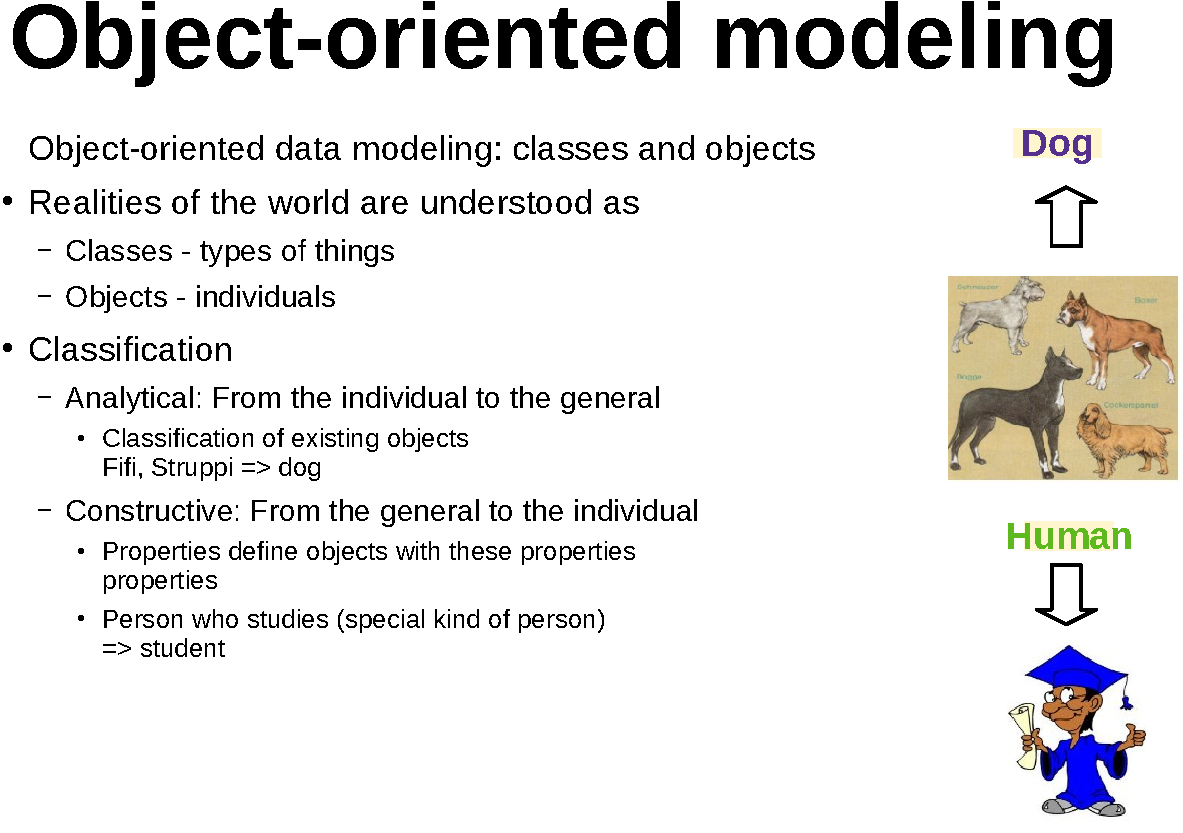
\includegraphics[page=1, width=0.7\linewidth]{img/out.pdf}}
    \caption{Pictures and tool-accessible text placed freehand on a slide}
    \label{fig:freehand}
\end{figure}

The words "Dog" and "Human" can be found by assisting tools. The arrows and the content of the small pictures are not accessible. 
Intended was an additional visualization of the concepts which are described in the text on the left side. It would be better to use diagrams whose structure is specified and which can be represented textually as introduced in the pattern \patternTwoInline.




The author of the following slide (Fig.~\ref{fig:table}) has inserted a table as an image on the slide. Arrows point to areas of the image and link explanations to the actual elements of the table.




\begin{figure}[ht!]
    \centering
    \fbox{\includegraphics[page=2, width= \linewidth]{img/out.pdf}}
    \caption{Table included as an image and mixed with textual information on a slide (image source: www.onlinemathlearning.com/)}
    \label{fig:table}
\end{figure}

The table is not accessible for the visually impaired. Explanations are extracted as text by assistive systems. The assignments and the table cannot be extracted. It is better to insert the table as a textual table. 
Explanations should also be assigned to the contents of the table as text.


Markdown is designed to use a minimal set of tags. Hence, it is easier to parse when access is done via text-to-speech or is read on a Braille display. 
Tools like Pandoc\footnote{\url{https://pandoc.org/}} can convert markdown text in a variety of formats like PDF, \ac{html} and office formats. As a result, it is possible to provide the clean text with the content for \ac{bvi} students and to give the others rendered outputs (e.g., PDF).

\newpage
Listing \ref{lst:table} shows the Markdown text which is rendered into the slide shown in Fig.~\ref{fig:table} using Pandoc.  


\begin{lstlisting}[label = lst:table, caption = Markdown of the slide in Fig~\ref{fig:table}]
# Boolean Operations
Operation: Conjunction
Operation name: AND
Input Variables: P, Q
Operation formula: $P \land Q$ 

Truth table:
| P | Q | P AND Q |
|---|---|-----|
| 0 | 0 | 0   |
| 0 | 1 | 0   |
| 1 | 0 | 0   |
| 1 | 1 | 1   |
\end{lstlisting}


This markdown is then converted into a slide in PDF using Pandoc with a user defined \LaTeX Beamer template accomplishing the CI specifications of the university.
\begin{figure}
    \centering
    \fbox{\includegraphics[page=2, width=0.8\linewidth]{img/Slides_Template.pdf}
    }
    \caption{Slide generated from markdown text}
    \label{fig:slideexample}
\end{figure}

The slides have the usual layout for sighted students.  
The markdown text is provided for the visually impaired and is easily accessible for them using assistive technologies. 


\subsection*{Consequences}



% Benefits
\renewcommand{\labelenumi}{$+$}
\begin{enumerate}
   \item Textual descriptions of graphics make them accessible for \ac{bvi} learners
\item Various output channels such as Braille displays or text-to-speech can be used by \ac{bvi} learners
\item Authors are encouraged to focus on the core content of the teaching materials
\item pure text based representations are independent from proprietary office tools and incompatibility problems can be avoided 
 
\end{enumerate}

% Liabilities
\renewcommand{\labelenumi}{$-$}
\begin{enumerate}
\item The creation of teaching materials takes longer
    \item Tool chains must be set up to generate teaching materials for sighted people
\item Changes and corrections are more time-consuming during creation because the tool chain for generating teaching materials for sighted people must be triggered again and again
\item Free manual placement of graphics on slides and other teaching materials is not possible
    \item Inserting content such as tables as screen shots from textbooks or websites should be avoided, but this leads to more work because the content has to be rewritten in text form
\item Graphic design options such as placing arrows over graphics to visualize relationships are limited
\end{enumerate}
 
\subsection*{Related Work}

Prior research has demonstrated that single-source authoring can enable
accessible learning materials for \ac{bvi} students in STEM.
The \emph{PreTeXt} project illustrates how semantically structured source files
can be transformed into multiple accessible outputs, including web, EPUB, and
Braille, while maintaining consistency across modalities
\cite{Austin2024PreTeXt}. 

Complementary studies on lightweight markup (e.g., R
Markdown) show that such workflows reduce authoring overhead and generate
accessible HTML and PDF outputs that integrate well with screen readers
\cite{Seo2019RMarkdown}. 

For mathematical content, web-based outputs can rely
on MathJax together with the Speech Rule Engine to provide adaptable
accessibility features such as structural navigation and speech rendering,
making them effective for non-visual exploration
\cite{CervoneSorge2019W4A}. 

When PDF is required, \LaTeX-based tool chains can
embed tagged formulae to improve screen-reader access; however, these retrofits
remain more fragile than web-first alternatives
\cite{Armano2018LaTeXPDF}.

